\chapter{2021年「大学物理1」\hdu 期末试题}
\date{2021年6月??日}{大学物理教学团队}{A0715011}
{未央物理讲师 \href{https://qm.qq.com/q/UPbGudx8cK}{\textbf{Axia}}}
{\qrcode{https://qm.qq.com/q/asJiytD5pC}}{「未央」HDU 物理营}
{\qrcode{http://weixin.qq.com/r/mhKYgFTEMQlOrRDj90eI}}{未央学社公众号}
\section{选择}
\begin{choice}{D}{}
 一质点在平面上做一般曲线运动，其瞬时速度为$\boldsymbol{v}$，瞬时速率为$v$，某一时间内的平均速度为$\overline{\boldsymbol{v}}$，平均速率为$\overline{v}$，它们之间的关系必定有：
\begin{tasks}(4)
\task $\left|\boldsymbol{v}\right|=v,\ \left|\overline{\boldsymbol{v}}\right|=\boldsymbol{v}$
\task $\left|\boldsymbol{v}\right|\neq v,\ \left|\overline{\boldsymbol{v}}\right|=\boldsymbol{v}$
\task $\left|\boldsymbol{v}\right|\neq v,\ \left|\overline{\boldsymbol{v}}\right|\neq\boldsymbol{v}$
\task $\left|\boldsymbol{v}\right|=v,\ \left|\overline{\boldsymbol{v}}\right|\neq\boldsymbol{v}$
\end{tasks}
\end{choice}
\begin{choice}{C}{}
人造地球卫星，绕地球作椭圆轨道运动，地球在椭圆的一个焦点上，则卫星的
\begin{tasks}(2)
\task 动量不守恒，动能守恒
\task 动量守恒，动能不守恒
\task 对地心的角动量守恒，动能不守恒
\task 对地心的叫动量不守恒，动能守恒
\end{tasks}
\end{choice}
\begin{choice}{D}{}
已知两个物体$A$和$B$的质量以及他们的速率都不相同，若物体$A$的动量在数值上比物体$B$的大，则$A$的动能$E_{k_A}$与$B$的动能$E_{k_B}$之间
\begin{tasks}(4)
\task $E_{k_B}$一定大于$E_{k_A}$
\task $E_{k_B}$一定小于$E_{k_A}$
\task $E_{k_B}=E_{k_A}$
\task 不能判定谁大谁小
\end{tasks}
\end{choice}

\hspace{-2.16em}
\begin{minipage}{0.67\textwidth}
    \begin{choice}{B}{}
    如图所示，一轻绳跨过一个定滑轮，两端各系一个质量分别为$m_1$和$m_2$的重物，且$m_1>m_2$，滑轮质量及轴上摩擦均不计，此时重物的加速度的大小为$a$.今用一竖直向下的恒力$F=m_1g$代替质量为$m_1$的物体，可得质量为$m_2$的重物的加速度的大小为$a^{\prime}$，则
    \begin{tasks}(4)
        \task $a^{\prime}=a$
        \task $a^{\prime}>a$
        \task $a^{\prime}<a$
        \task 不能确定
    \end{tasks}
    \end{choice}
\end{minipage}
\hfill
\begin{minipage}[c]{0.33\textwidth}
\begin{center}
    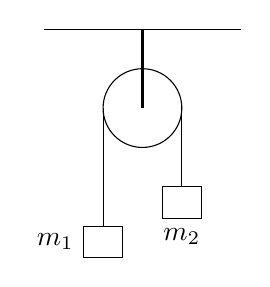
\begin{tikzpicture}[scale=0.5]
        \centering
        \draw (1,6)--(6,6);
        \draw[very thick] (3.5,6)--(3.5,4);
        \draw (2.5,4)--(2.5,1);
        \draw (4.5,4)--(4.5,2);
        \draw (3.5,4) circle (1);
        \draw (2,0.2)--(2,1)--(3,1)--(3,0.2)--(2,0.2);
        \draw (4,1.2)--(4,2)--(5,2)--(5,1.2)--(4,1.2);
        \coordinate [label=left:{$m_1$}] (m1) at (2,0.6);
        \coordinate [label=below:{$m_2$}] (m2) at (4.5,1.2);
    \end{tikzpicture}
\end{center}
\end{minipage}

\begin{choice}{B}{}
电荷面密度为$+\sigma$的两块“无限大”均匀带电的平行平板如图放置，其周围空间各点电场强度$\boldsymbol{E}$随位置坐标$x$变化的关系曲线为（设场强方向向右为正、向左为负）

\begin{minipage}{0.6\linewidth}
    \begin{minipage}{0.48\linewidth}
    \begin{tikzpicture}[scale=0.4]
    \centering
    \draw [->](-5,0)--(5,0);
    \draw [->](0,-3)--(0,4);
    \draw [thick](-4,1)--(-2,1);
    \draw [thick](-2,2)--(2,2);
    \draw [thick](2,1)--(4,1);
    \draw [densely dotted](-2,0)--(-2,2);
    \draw [densely dotted](2,0)--(2,2);
    \coordinate [label=right:{$E$}] (E) at (0,4);
    \coordinate [label=below:{$x$}] (x) at (5,0);
    \coordinate [label=above:{$\sigma/\varepsilon_0$}] (e1) at (1,2);
    \coordinate [label=above:{$\sigma/2\varepsilon_0$}] (e2) at (3,1);
    \coordinate [label=below:{$-a$}] (-a) at (-2,0);
    \coordinate [label=below:{$+a$}] (+a) at (2,0);
    \coordinate [label=below:{A}] (a) at (0,-3.5);
    \end{tikzpicture}
    \end{minipage}
    \hfill
    \begin{minipage}{0.48\linewidth}
    \begin{tikzpicture}[scale=0.4]
    \centering
    \draw [->](-5,0)--(5,0);
    \draw [->](0,-3)--(0,4);
    \draw [thick](-4,-2)--(-2,-2);
    \draw [thick](-2,0)--(2,0);
    \draw [thick](2,2)--(4,2);
    \draw [densely dotted](-2,-2)--(-2,0);
    \draw [densely dotted](2,0)--(2,2);
    \coordinate [label=right:{$E$}] (E) at (0,4);
    \coordinate [label=below:{$x$}] (x) at (5,0);
    \coordinate [label=above:{$\sigma/2\varepsilon_0$}] (e2) at (3,2);
    \coordinate [label=below:{$-a$}] (-a) at (-2,0);
    \coordinate [label=below:{$+a$}] (+a) at (2,0);
    \coordinate [label=below:{B}] (b) at (0,-3.5);
    \end{tikzpicture}
    \end{minipage}
    \vfill
    \begin{minipage}{0.48\linewidth}
    \begin{tikzpicture}[scale=0.4]
    \centering
    \draw [->](-5,0)--(5,0);
    \draw [->](0,-3)--(0,4);
    \draw [thick](-4,0)--(-2,0);
    \draw [thick](-2,2)--(2,2);
    \draw [thick](2,0)--(4,0);
    \draw [densely dotted](-2,0)--(-2,2);
    \draw [densely dotted](2,0)--(2,2);
    \coordinate [label=right:{$E$}] (E) at (0,4);
    \coordinate [label=below:{$x$}] (x) at (5,0);
    \coordinate [label=above:{$\sigma/\varepsilon_0$}] (e1) at (1,2);
    \coordinate [label=below:{$-a$}] (-a) at (-2,0);
    \coordinate [label=below:{$+a$}] (+a) at (2,0);
    \coordinate [label=below:{C}] (c) at (0,-3.5);
    \end{tikzpicture}
    \end{minipage}
    \hfill
    \begin{minipage}{0.48\linewidth}
    \begin{tikzpicture}[scale=0.4]
    \centering
    \draw [->](-5,0)--(5,0);
    \draw [->](0,-3)--(0,4);
    \draw [thick](-4,2)--(-2,2);
    \draw [thick](-2,0)--(2,0);
    \draw [thick](2,2)--(4,2);
    \draw [densely dotted](-2,0)--(-2,2);
    \draw [densely dotted](2,0)--(2,2);
    \coordinate [label=right:{$E$}] (E) at (0,4);
    \coordinate [label=below:{$x$}] (x) at (5,0);
    \coordinate [label=above:{$\sigma/\varepsilon_0$}] (e1) at (3,2);
    \coordinate [label=below:{$-a$}] (-a) at (-2,0);
    \coordinate [label=below:{$+a$}] (+a) at (2,0);
    \coordinate [label=below:{D}] (d) at (0,-3.5);
    \end{tikzpicture}
    \end{minipage}
    \end{minipage}
    \hfill
    \begin{minipage}{0.4\linewidth}
    \begin{tikzpicture}[scale=0.8]
    \centering
    \draw [->](-4,0)--(4,0);
    \draw [->](0,-3)--(0,3);
    \draw [thick](-2,-2)--(-2,2);
    \draw [thick](2,-2)--(2,2);
    \draw [densely dotted](-2,-3)--(-2,3);
    \draw [densely dotted](2,-3)--(2,3);
    \coordinate [label=right:{$y$}] (y) at (0,3);
    \coordinate [label=below:{$x$}] (x) at (4,0);
    \coordinate [label=below left:{$+\sigma$}] (sigma) at (-2,3);
    \coordinate [label=below right:{$+\sigma$}] (sigma) at (2,3);
    \coordinate [label=below left:{$-a$}] (-a) at (-2,0);
    \coordinate [label=below right:{$+a$}] (+a) at (2,0);
    \coordinate [label=below left:{$O$}] (+a) at (0,0);
    \end{tikzpicture}
    \end{minipage}
\end{choice}

\begin{choice}{D}{}
一个带正电荷的质点，在电场力作用下从$A$点出发经$C$点运动到$B$点，其运动轨迹如图所示.已知质点运动的速率是递减的，下面关于$C$点场强方向的四个图示中正确的是
\end{choice}
\vspace{5em}
% \begin{minipage}{0.5\linewidth}
%  \begin{minipage}{0.48\linewidth}
%   \centerline{\includegraphics[width=2cm]{图1-6A.png}}
%   \centerline{A}
%  \end{minipage}
%  \hfill
%  \begin{minipage}{0.48\linewidth}
%   \centerline{\includegraphics[width=2cm]{图1-6B.png}}
%   \centerline{B}
%  \end{minipage}
% \end{minipage}
% \begin{minipage}{0.5\linewidth}
%  \begin{minipage}{0.48\linewidth}
%   \centerline{\includegraphics[width=2cm]{图1-6C.png}}
%   \centerline{C}
  
%  \end{minipage}
%  \hfill
%  \begin{minipage}{0.48\linewidth}
%   \centerline{\includegraphics[width=2cm]{图1-6D.png}}
%   \centerline{D}
%  \end{minipage}
% \end{minipage}

\hspace{-2.16em}
\begin{minipage}{0.67\textwidth}
    \begin{choice}{D}{}
        在磁感应强度$\boldsymbol{B}$的均匀磁场中作一半径为$r$的半球面$S$，$S$边线所在平面的法线方向单位矢量$\boldsymbol{n}$与$\boldsymbol{B}$的夹角为$\alpha$，则通过半球面$S$的磁通量（取弯曲面向外为正）为
        \begin{tasks}(4)
        \task $\pi r^2B$
        \task $2\pi r^2B$
        \task $-\pi r^2B\sin\alpha$
        \task $-\pi r^2B\cos\alpha$
        \end{tasks}
    \end{choice}
\end{minipage}
\hfill
\begin{minipage}[c]{0.33\textwidth}
\begin{center}
    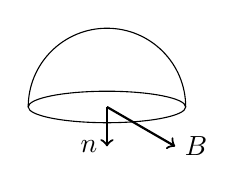
\begin{tikzpicture}
        \draw (1,0) arc (0:180:1);
        \draw (0,0) ellipse (1 and 0.2);
        \draw [thick,->] (0,0)--(0,-0.5);
        \draw [thick,->] (0,0)--(0.86603,-0.5);
        \coordinate[label=left:$\boldsymbol{n}$] (n) at (0,-0.5);
        \coordinate[label=right:$\boldsymbol{B}$] (B) at (0.86603,-0.5);
    \end{tikzpicture}
\end{center}
\end{minipage}

\begin{choice}{B}{}
距一根载有电流为$3\times 10^4\mathrm{A}$的长直载流电线$1\mathrm{m}$处的磁感应强度的大小为（已知真空中的磁导率$\mu_0=4\pi\times 10^{-7}\mathrm{T\cdot m/A}$）
\begin{tasks}(4)
    \task $3\times 10^{-5}\mathrm{T}$
    \task $6\times 10^{-3}\mathrm{T}$
    \task $1.9\times 10^{-2}\mathrm{T}$
    \task $0.6\mathrm{T}$
\end{tasks}
\end{choice}
\begin{choice}{B}{}
所讨论的空间处在稳恒磁场中，对于安培环路定律的理解，正确的是
\begin{tasks}(2)
    \task 若$\oint\limits_L\vv{B}\cdot\d\vv{l}=0$，则必定$L$上$\vv{B}$处处为零.
    \task 若$\oint\limits_L\vv{B}\cdot\d\vv{l}=0$，则$L$所包围电流的代数和为零.
    \task 若$\oint\limits_L\vv{B}\cdot\d\vv{l}=0$，则必定$L$不包围电流.
    \task 回路$L$上各点的$B$仅与所包围的电流有关.
\end{tasks}
\end{choice}
\section{填空}
\begin{exercise}{3}{}
    一质点沿$x$轴作直线运动，它的运动学方程为$x=3+5t+6t^2-t^3\ \boldsymbol{\mathrm{(SI)}}$，则
    \begin{enumerate}[(1)]
        \item 质点在$t=0$时刻的速度$\boldsymbol{v}_0=$\underline{\hbox to 20mm{}}.
        \item 加速度为零时，该质点的速度$\boldsymbol{v}=$\underline{\hbox to 20mm{}}.
    \end{enumerate}
\end{exercise}

\hspace{-2.16em}
\begin{minipage}{0.67\textwidth}
    \begin{exercise}{4}{}
        质量相等的两物块$A$和$B$，分别固定在弹簧的两端，竖直放在光滑水平面$C$上，如图所示，弹簧的质量与物体$A$、$B$的质量相比可以忽略不计.若把支持面$C$迅速移走，则在移开的一瞬间，$A$的加速度大小$a_A=$\underline{\hbox to 10mm{}}，$B$的加速度大小$a_B=$\underline{\hbox to 10mm{}}.
        \end{exercise}
\end{minipage}
\hfill
\begin{minipage}[c]{0.33\textwidth}
\begin{center}
    \begin{tikzpicture}
    
    \end{tikzpicture}
\end{center}
\end{minipage}

\hspace{-2.16em}
\begin{minipage}{0.67\textwidth}
\begin{exercise}{3}{}
    真空中，一边长为$a$的正方形平板上均匀分布着电荷$q_1$在其中垂线上距离平板$d$出放一点电荷$q_0$，如图所示.在$d$与$a$满足\underline{\hbox to 10mm{}}条件下，$q_0$所受电场力可写成$q_0q/\ab(4\pi\varepsilon_0d^2s)$
\end{exercise}
\end{minipage}
\hfill
\begin{minipage}[c]{0.33\textwidth}
\begin{center}
    \begin{tikzpicture}
    
    \end{tikzpicture}
\end{center}
\end{minipage}

\begin{exercise}{3}{}
    质量为$m$的质点以 速度$\boldsymbol{v}$沿一直线运动，则它对直线外垂直距离为$d$的一点的角动量大小是\underline{\hbox to 20mm{}}.
    \end{exercise}

\begin{exercise}{3}{}
由一根绝缘细线围成的边长为$l$的正方形线框，使它均匀带电，其电荷线密度为$\lambda$，则在正方形中心处的电场强度的大小$E=$\underline{\hbox to 20mm{}}.
\end{exercise}

\hspace{-2.16em}
\begin{minipage}{0.67\textwidth}
    \begin{exercise}{3}{}
        图中所示为静电场的等（位）线图，已知$U_1>U_2>U_3$.在图上画出$a$、$b$两点的电场强度方向，并比较它们的大小.$E_a$\underline{\hbox to 10mm{}}$E_b$（填<、=、>）.
    \end{exercise}
\end{minipage}
\hfill
\begin{minipage}[c]{0.33\textwidth}
\begin{center}
    \begin{tikzpicture}
    
    \end{tikzpicture}
\end{center}
\end{minipage}
\vspace{1em}

\hspace{-2.16em}
\begin{minipage}{0.67\textwidth}
    \begin{exercise}{3}{}
        如图所示，电荷$q(>0)$均匀地分布在一个半径为$R$的薄球壳外表面上，若球壳以恒角速度$\omega_0$绕$z$轴转动，则沿着$z$轴从$-\infty$到$+\infty$磁感强度的线积分等于\underline{\hbox to 20mm{}}.（提示：安培环路定理）
        \end{exercise}
\end{minipage}
\hfill
\begin{minipage}[c]{0.33\textwidth}
\begin{center}
    \begin{tikzpicture}
    
    \end{tikzpicture}
\end{center}
\end{minipage}

\hspace{-2.16em}
\begin{minipage}{0.67\textwidth}
    \begin{exercise}{3}{}
        在阴极射线管（电子以$v$的速度水平向右出射）的上方平行管轴方向上放置一长直载流导线，电流方向如图所示，那么射线应\underline{\hbox to 20mm{}}（向下或向上）偏转.
        \end{exercise}
\end{minipage}
\hfill
\begin{minipage}[c]{0.33\textwidth}
\begin{center}
    \begin{tikzpicture}
    
    \end{tikzpicture}
\end{center}
\end{minipage}

\section{计算}
\begin{exercise}{9}{}
一敞顶电梯以恒定速率$v=10\mathrm{m/s}$上升.当电梯高地面$h=10\mathrm{m}$时，一小孩竖直向上抛出一球.球相对于电梯初速率$v=20\mathrm{m/s}$，试问：
\begin{enumerate}[(1)]
    \item 从地面算起，球能达到的最大高度为多大？
    \item 抛出后经过多长时间再回到电梯上？
\end{enumerate}
\end{exercise}'

\hspace{-2.16em}
\begin{minipage}{0.67\textwidth}
    \begin{exercise}{8}{}
        如图所示，一质量为$m$的物体与绕在定滑轮上的绳子相联，绳子质量可以忽略，它与定滑轮之间无滑动.假设定滑轮质量为$M$、半径为$R$，其转动惯量为$\frac{1}{2}MR^2$，滑轮轴光滑.试求该物体由静止开始下落的过程中，下落速率与时间的关系.
        \end{exercise}
\end{minipage}
\hfill
\begin{minipage}[c]{0.33\textwidth}
\begin{center}
    \begin{tikzpicture}
    
    \end{tikzpicture}
\end{center}
\end{minipage}

\begin{exercise}{8}{}
一均匀木杆，质量为$m_1=1\mathrm{kg}$，长$l=0.4\mathrm{m}$，可绕通过它的中点且与杆身垂直的光滑水平固定轴在竖直平面内转动.设杆静止于竖直位置时，一质量为$m_2=10\mathrm{g}$的子弹在距杆中点$\frac{l}{4}$处穿透木杆（穿透所用时间不计）,子弹初速度的大小$v_0=200\mathrm{m/s}$，方向与杆和轴均垂直.穿出后子弹速度大小减为$v=50\mathrm{m/s}$，但方向未变.求子弹刚穿出的瞬时，杆的角速度的大小（木杆绕通过中点的垂直轴的转动惯量$J=\frac{1}{12}ml^2$）.
\end{exercise}
\begin{exercise}{8}{}
一内半径为$a$、外半径为$b$的金属球壳，带有电荷$Q$,在球壳空腔内距离球心$r$处有一点电荷$q$.设无限远处为电势零点，试求：
\begin{enumerate}[(1)]
    \item 球壳内外表面上的电荷；
    \item 球心$O$点处，由球壳内表面上电荷产生的电势；
    \item 球心$O$点处的总电势.
\end{enumerate}
\end{exercise}

\hspace{-2.16em}
\begin{minipage}{0.67\textwidth}
    \begin{exercise}{5}{}
        三根平行长直导线在同一平面内，$1$、$2$和$2$、$3$之间距离都是$d=3\mathrm{cm}$，其中电流$I_1=I_2$，$I_3=-\left(I_1+I_2\right)$，方向如图.试求在该平面内$B=0$的直线的位置.
        \end{exercise}
\end{minipage}
\hfill
\begin{minipage}[c]{0.33\textwidth}
\begin{center}
    \begin{tikzpicture}
    
    \end{tikzpicture}
\end{center}
\end{minipage}

\begin{exercise}{10}{}
两根平行无限长直导线相距为$d$，载有大小相等方向相反的电流$I$，电流变化率$\frac{\mathrm{d}I}{\mathrm{d}t}=\alpha>0$.一个边长为$d$的正方形线圈位于导线平面内与一根导线相距$d$，如图所示.求线圈中的感应电动势，并说明线圈中的感应电流是顺时针还是逆时针方向.
\end{exercise}
